
\section{Microcirculatory system}

In this section the hand will be used as an example point, to describe the microcirculatory system. 

The heart and larger arteries and veins are what we usually associate with the cardiovascular system, but actually those are only mainly used for transport of blood. Instead it is the capillaries, that permeate most tissues, that is responsible for the perfusion of tissue. These are the only vessels that permit exchange between the vessel and the surrounding interstitial fluids.    
Capillaries are made not of single individual fluid conductors like veins and arteries, but instead formed capillary beds. Here they work as a interconnected network of vessels. As mentioned before the arterioles divide into dozen of capillaries which then merge into a venule, after the blood has been de-oxygenated. A capillary is divided into two segments, first the metarteriole and second the capillary. The blood flow between arterioles and venules can also be a direct connection, made by an arteriovenous anastomosis. This works as a bypass diverting blood flow around the capillary bed. An example of the structure of the capillary bed can be seen on \cref{fig:beds}.\cite{martini2012}
\begin{figure}[H]                                         
	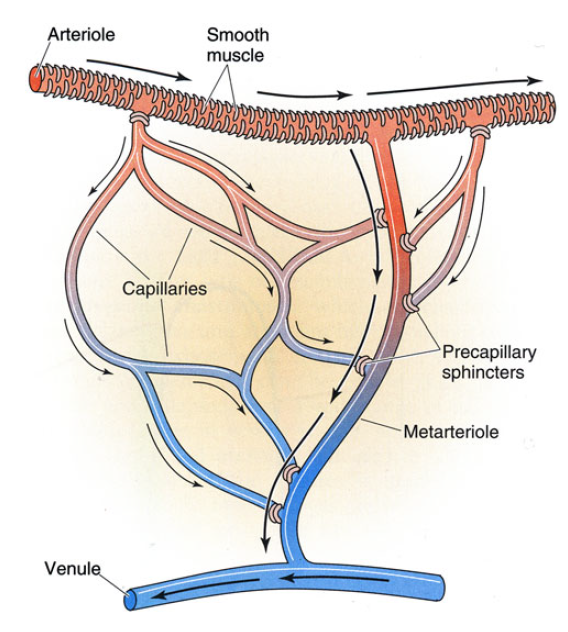
\includegraphics[width=.6\textwidth]{figures/capillary_bed}  
	\caption{The basic structure of a capillary bed, with arteriole on the left side of the bed and a venule on the right.}
	\label{fig:beds}  
\end{figure}          

Each capillary entrance is controlled by a precapillary sphincter, which is composed of smooth muscle cells, that are able to contract or relax and thereby limit access of blood flow to certain capillaries. The blood flows relatively slow within the capillaries giving time for the two way exchange of nutrients and wastes. \cite{martini2012}

\subsection{Vasmotion}

The flow within the capillaries varies. This is due to the earlier mentioned precapillary sphincters contracts and relaxes. The opening and closing of sphincters is part of the autoregulation process performed at a local level, to control the blood flow. Local changes in concentration of chemicals and interstitial fluids eg. dissolved oxygen concentrations in tissue cause the sphincters to dilate permitting a greater flow of blood to the area. The cardiovascular system does not contain blood enough for every vessel a capillary beds to be filled with blood. Therefore only 25 perfect of the vessels in a capillary bed contains blood, and vessels activity needs to be well coordinated.\cite{martini2012}

Under normal circumstances cardiac output remains stable and the control of local blood flow happens through local peripheral resistance within local tissues. The regulation of cardiovascular activity is controlled by local homeostatic mechanism. These make sure that demands such as oxygen and nutrients are meet and wastes are disposed.  \cite{martini2012} 

Factors that promote dilation is called vasodilators and can be some of the following: 
\begin{itemize}
	\item Decreased oxygen level or increased CO2 level
	\item Lactic acid or other acids generated from tissue cells
	\item Nitric oxide NO released from endothelial cells
	\item Rising concentrations of potassium ions or hydrogen ions in the interstitial fluid.
	\item Chemicals released during local inflammation
	\item Elevated local temperature
\end{itemize} 

A vasodialation will result in increased oxygen, nitrients, buffers released to recreate homeostasis.
Factors that stimulate contriction is called vasoconstricters and can happen due to following:

\begin{itemize}
	\item Damaged tissue
	\item Aggregating platelets 
\end{itemize}

Factors that affect tissue perfusion is cardiac output, peripheral resistance and blood pressure\cite{martini2012}. 





